\section{SW-Konzeption sowie Basisfunktionalitäten}
\label{sec:konzeption-kommunikation}
%
Das Konzept besteht aus drei Schichten. Eine dieser Schichten ist die Geschwindigkeitsregelung. Zudem gibt es die Kameraverarbeitung und die Trajektorienplanung. 
Zusammen %sollen 
bieten sie die Grundlage für das Fahrzeug, damit es dazu in der Lage ist, eine Strecke entlang zu fahren die durch weiße Linien begrenzt ist.

\begin{wrapfigure}[]{R}{0.4\textwidth}
    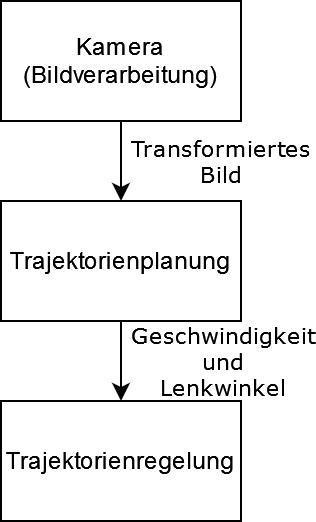
\includegraphics[width=0.4\textwidth]{bilder/DreiSchichten.png}
    \caption{Das Konzept in drei \\ Schichten unterteilt%
             \label{fig:dreiSchichten}}
\end{wrapfigure}

\begin{description}
    \item [Die Kameraverarbeitung]
    gibt ein bereits vorverarbeites, transformiertes Bild vor.
    \item [Die Trajektorienplanung]
    nimmt das Bild aus der Kameraverarbeitung und erstellt darin eine Trajektorie die eine Geschwindigkeit und eine Fahrtrichtung vorgibt.
    \item [Die Geschwindigkeitsregelung]
    bekommt die SOLL-Geschwindigkeit und den SOLL-Lenkwinkel von der Trajektorienplanung und regelt die IST-werte ein. 
\end{description}

Der Teil dieser Arbeit beschäftigt sich vor allem mit der Geschwindigkeitsregelung und anderen Basisfunktionalitäten. 
Der Geschwindigkeitsregler soll auf Basis der durch die Radodometrie gemessenen Radgeschwindigkeit und der durch die IMU gemessenen Beschleunigung die Geschwindigkeit des Fahrzeuges regeln. Die Implementierung der Regelung benötigt Vorarbeit denn die Odometrie des Fahrzeugs gibt eine Geschwindigkeit an, die IMU eine Beschleunigung. 
Damit nun beide Signale im Bezug zueinander genommen werden können muss entweder die Geschwindigkeit der Odometrie differenziert werden oder die Beschleunigung der Imu integriert. 
Beide Ansätze werden in dieser Dokumentation verfolgt und auf ihre Eignung getestet. Zuvor wurden jedoch ein paar Tests, mit der Imu und der Odometrie gemacht. 
Das Signal der Imu ist noch mit einer der Gravitationsbeschleunigung behaftet und zudem liegt das Koordinatensystem des Beschleunigungssensor nicht parallel dem des Fahrzeugs, näheres dazu in Abschnitt \ref{sec:imu}. 

\subsubsection{Konzept der Geschwindigkeitsregelung}
Die Regelung soll als Eingangssignal eine SOLL-Geschwindigkeit $v_{soll}$ von der Trajektorienplanung bekommen. Die Odometrie liefert eine Radgeschwindigkeit $v_{rad}$. Aus der Differenz von $v_{soll}$ und $v_{rad}$ lässt sich eine Regelabweichung $e$ bestimmen. Wenn die Die Differenz zwischen der Odometrie und den Werten der Imu sollen einen IST-Schlupf erzeugen.

\textcolor{red}{Wenn Sie da eine Regelung vornehmen wollen stellt sich die Frage: Was davon ist das Soll-Signal und was ist das IST-Signal von Geschwindigkeit und Beschleunigung...??? Für mich sind bis zu diesem Punkt in der Doku das jeweils \glqq{}Mess-Signale / Ist-Signale\grqq{}...! Für eine Regelung fehlt also nach wie vor eine Soll-Vorgabe...!}

\begin{figure}
    \centering
    \hspace*{-0.4cm}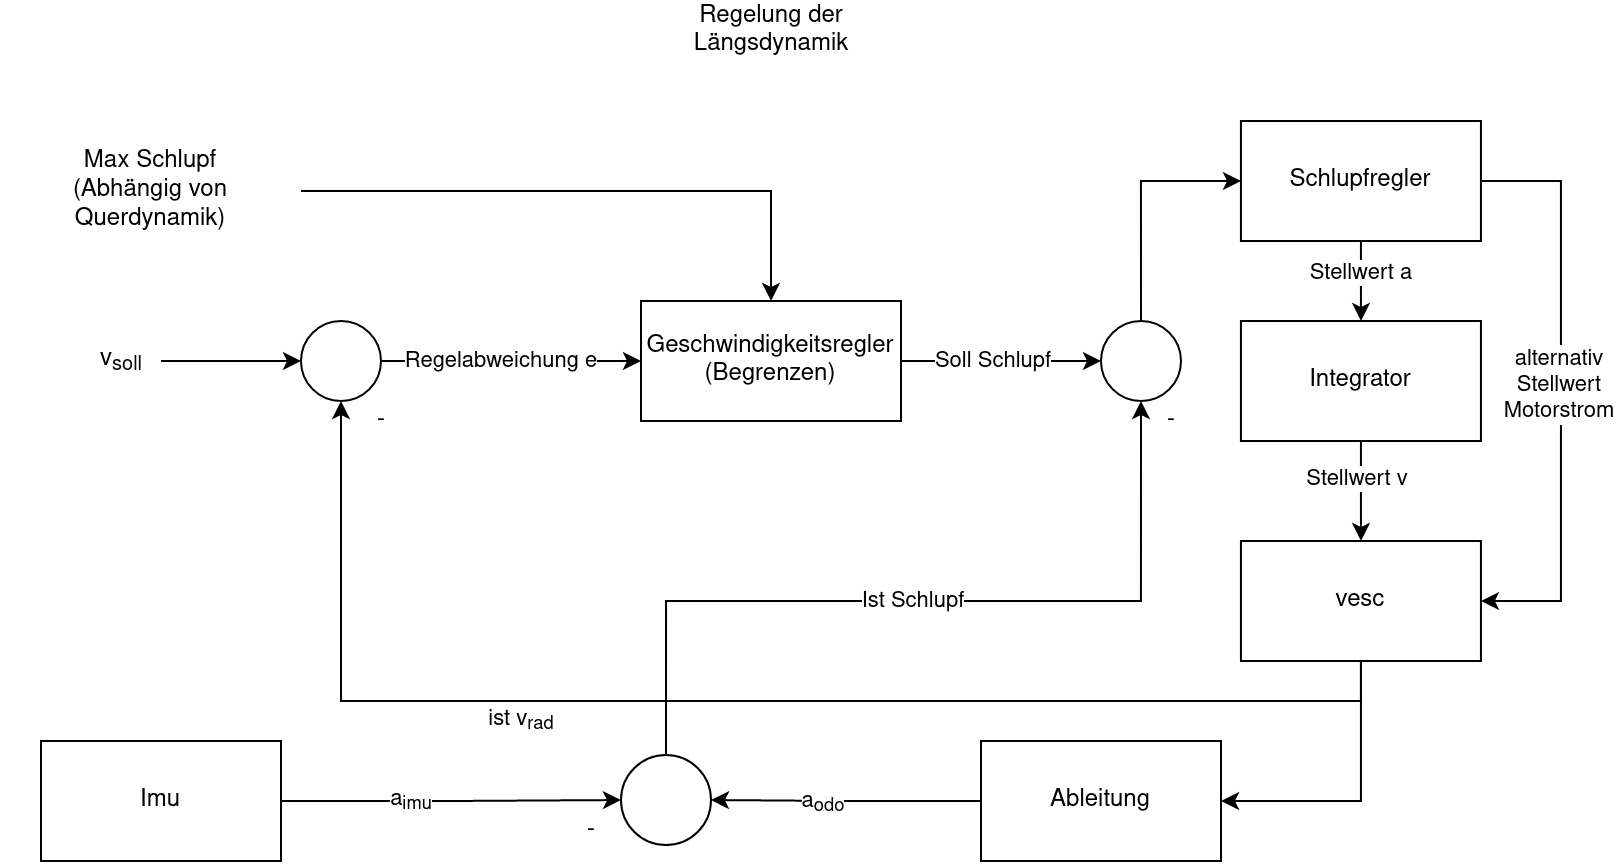
\includegraphics[width=1.05\textwidth]{bilder/SEP-Plan.png}
    \caption{Diagramm der Regelung}
    \label{fig:diagramRegelung}
\end{figure}

\subsection{Verbindung ROS Systeme}
In ROS 1 ist es noch notwendig ein paar Variablen im Terminal zu exportieren damit sich zwei Systeme im selben Netzwerk verbinden können.

Dazu stellt diese Dokumentation ein Skript zur Verfügung, um den Laptop mit dem Jetson, dem Computer des Autos, zu verbinden; das sogenannte  ROS-Master/Slave System. 
Mit Hilfe des Skripts gelingt es Skripte an einem anderen Rechner/System zu schreiben und zu starten.
%Dazu wurde ein kleines Skript geschrieben um den Laptop mit dem Jetson, der Computer des Autos, zu verbinden. (ROS-
%Master/Slave System)
%Dadurch können Skripte an einem anderen System geschrieben und gestartet werden. 
%Sind -- z.B. bei einem Wettbewerb / Rennen -- häufiger kleinere Änderungen vorzunehmen, so steht mehr (dezentralisierte) Rechenleistung für diese Aufgabe zur Verfügung 
%kann auf mehr Rechenleistung zurückgegriffen werden und diese müssen dann 

\subsection{Skripte}
Für alle erstellten Tests und Funktionen gibt es jeweils die folgenden Skripte.

\begin{description}
\item[move\_base.py]
ist ein Skript dass das Fahrzeug linear bewegt.
Dieses Skript wartet auf ein Signal das entweder 0 ist um zu stoppen oder 1 um
mit einer vorher definierten Geschwindigkeit geradeaus zu fahren.
Dieses Skript ermöglicht einfache Tests für die Beschleunigungs- und Geschwindigkeitsmessung.

\item[imuorientation.py]
ist ein Skript dass die Werte der IMU als Durchschnittswerte in der Konsole ausgibt. Als Input dient nutzt das Programm den Topic der IMU\footnote{\url{http://docs.ros.org/en/melodic/api/sensor_msgs/html/msg/Imu.html}}. Das Skript errechnet die Durchschnittswerte über mehrere Zyklen, so soll verhindert werden das Ausreißer zu viel Einfluss auf das Ergebnis haben. Nach einer vorgegebenen Zeit stoppt das Programm und gibt die Werte in der Konsole aus. Die Ausgabe besteht dann aus:
\begin{itemize}
    \item xMean, yMean zMean
    \item orientationRollMean, orientationPitchMean, orientationYawMean
    \item amountAccelerationMean
\end{itemize}
Besonders interessant zum Kalibrieren ist hier der Wert \strong{amountAccelerationMean}, er gibt den Betrag des Beschleunigungsvektor an.  
Das Ergebnis dieses Vektors sollte stets die Erdbeschleunigung sein. Durch empirische Versuche wurden so Ungereimtheiten mit der Kalibrierung der IMU behoben. Weiter Informationen zur Kalibrierung in Abschnitt \ref{sec:KalibrierungImu}.

\item[imuTestWithRemovingGravity.py]
ist analaog zu dem \strong{imuorientation.py} Skript, zudem entfernt es noch die Erdbeschleunigung aus den Daten. Das Resultat muss dann 0 ergeben. Dazu verwendet das Skript Quaternionen-Multiplikation. 

\lstinputlisting[language=Python, linerange={71-78,81-92,106-112}]{skripte/imutestWithRemovingGravity.py}

Dadurch das 6-Achsen durch die IMU gegeben sind, die Beschleunigung und die Orientierung zum Erdkoordinatensystem, kann durch die Anwendung von Quaternionen-Multiplikation das Koordinatensystem auf das Erdkoordinatensystem transformiert werden. Anschließend muss nur die Gravitation als Vektor abgezogen werden und bei Bedarf das Koordinatensystem wieder zurück transformiert werden. Dieses Skript diente vor allem dazu, zu Testen wie die Erdbeschleunigung raus gerechnet werden kann. Die Ergebnisse dieses Skriptes dienten zur Vorlage des \strong{remove\_gravity\_from\_imu.py} und anschließend des \strong{RemoveGravityFromImu.cpp} Skripts.

\item[remove\_gravity\_from\_imu.py] erbt von \strong{imuorientation.py} teile des codes. Dieses Skript ist in der 


-Diverse Skripte Tests mit der IMU und der Odometrie durch zu führen
-Einmal wurde das Signal der IMU Integriert um aus der Beschleunigung eine Geschwindigkeit zu bekommen (Hier muss natürlich deutlich mehr Inhalt und Referenzen
rein.)
-Zum Schluss wurde das Signal der Odometrie Differenziert um aus der Geschwindigkeit
der Odometrie eine Beschleunigung zu bekommen. (Das war analog zum anderen und
hat deutlich weniger Aufwand gekostet, könnte natürlich aber auch weiter ausgeführt
werden)

\end{description}

\subsection{imu}
\label{sec:imu}
Wie in Abschnitt \ref{sec:VDI-Racer-Aufbau} beschrieben, besteht eine IMU aus mehreren Sensoren, die Fusioniert und Ausgewertet die Orientierung, lineare sowie angulare Beschleunigung ergeben. Die IMU gibt die tatsächliche Beschleunigung des Fahrzeugs wider. Sie kann in einem Regelkreis dazu verwendet werden, die SOLL-Beschleunigung/Geschwindigkeit mit den Werten der IMU zu vergleichen, um dann eine Entscheidung zu treffen, ob die Beschleunigung zu stark oder zu schwach ist für den derzeitigen Untergrund. So soll das durchrutschen der Reifen vermieden werden.

\subsubsection{Kalibrierung}
\label{sec:KalibrierungImu}
Eine Kalibrierung des Sensors ist unerlässlich, da durch die Fertigung stets Unterschiede zwischen jeden Sensor bestehen. Für die Kalibrierung ist das Skript verantwortlich das auf dem Arduino läuft, dieses wird bereits von dem \strong{mpu6050\_serial\_to\_imu} Paket bereitgestellt. Das Sript ist jedoch so geschrieben, das es nach dem Verbinden mit dem Rechner die IMU jedes mal automatisch neu Kalibriert. Das führt zu einer immer anderen Kalibrierung, die eventuell nicht gewünscht ist. Es soll verhindert werden das, sollte sich die IMU während der Fahrt neu verbinden, die Kalibrierung in einer Bewegung statt findet, oder die Lage des Fahrzeugs sich ändert. 

Das bedeutet, dass die Kalibrierung manuell stattfindet. Dazu werden die Werte aus der automatischen Kalibrierung genommen und in den Code fest implementiert. Das \strong{imuorientation.py} Skript hilft dabei, die Kalibrierung zu überprüfen. Durch Systematisches auswerten der Achsen indem die IMU entweder Horizontal, Vertikal oder Beides positioniert wird

\subsubsection{Probleme und Hürden}
\label{sec:imu-probleme}
Die meisten Sensoren sind mit einem Rauschen behaftet oder führen gerade an Extrempunkten zu unerwünschten Verhalten. Auch die IMU hat diese Probleme, weshalb der Ansatz die Beschleunigungswerte der IMU zu nutzen um eine Geschwindigkeit zu erhalten, zu einer stetig steigenden (oder abnehmenden) Geschwindigkeit führt. Diesen Effekt nennt man bei Beschleunigungssensoren drift. Der Drift führt dazu, das der Beschleunigungssensor immer eine kleine Kraft in eine beliebige Richtung erfährt, ob er nun Still liegt oder nicht. Durch das Kalibrieren wird dieser Drift so weit es geht reduziert. Jedoch entsteht dieser drift vor allem durch die Erdanziehung, die eine konstante Kraft auf den Sensor ausübt. Damit diese Kraft möglichst keine oder nur geringe Auswirkungen auf das Ergebnis hat, wird sie aus den Messwerten entfernt. 

Das \strong{gravity\_from\_imu\_remover.cpp} Skript ist eigens dafür verantwortlich, die Gravitation aus der IMU raus zu rechnen. Es hört auf das Topic der IMU, rechnet die Erdbeschleunigung als Vektor \begin{equation}
    \vec g = \left(\begin{array}{c} 0 \\ 0 \\ 9.81 \end{array}\right)
\end{equation}
raus und versendet dann die eigenen Daten wieder als Topic und stellt die Daten damit anderen Programmen zur Verfügung. 

\begin{figure}
    \centering
%    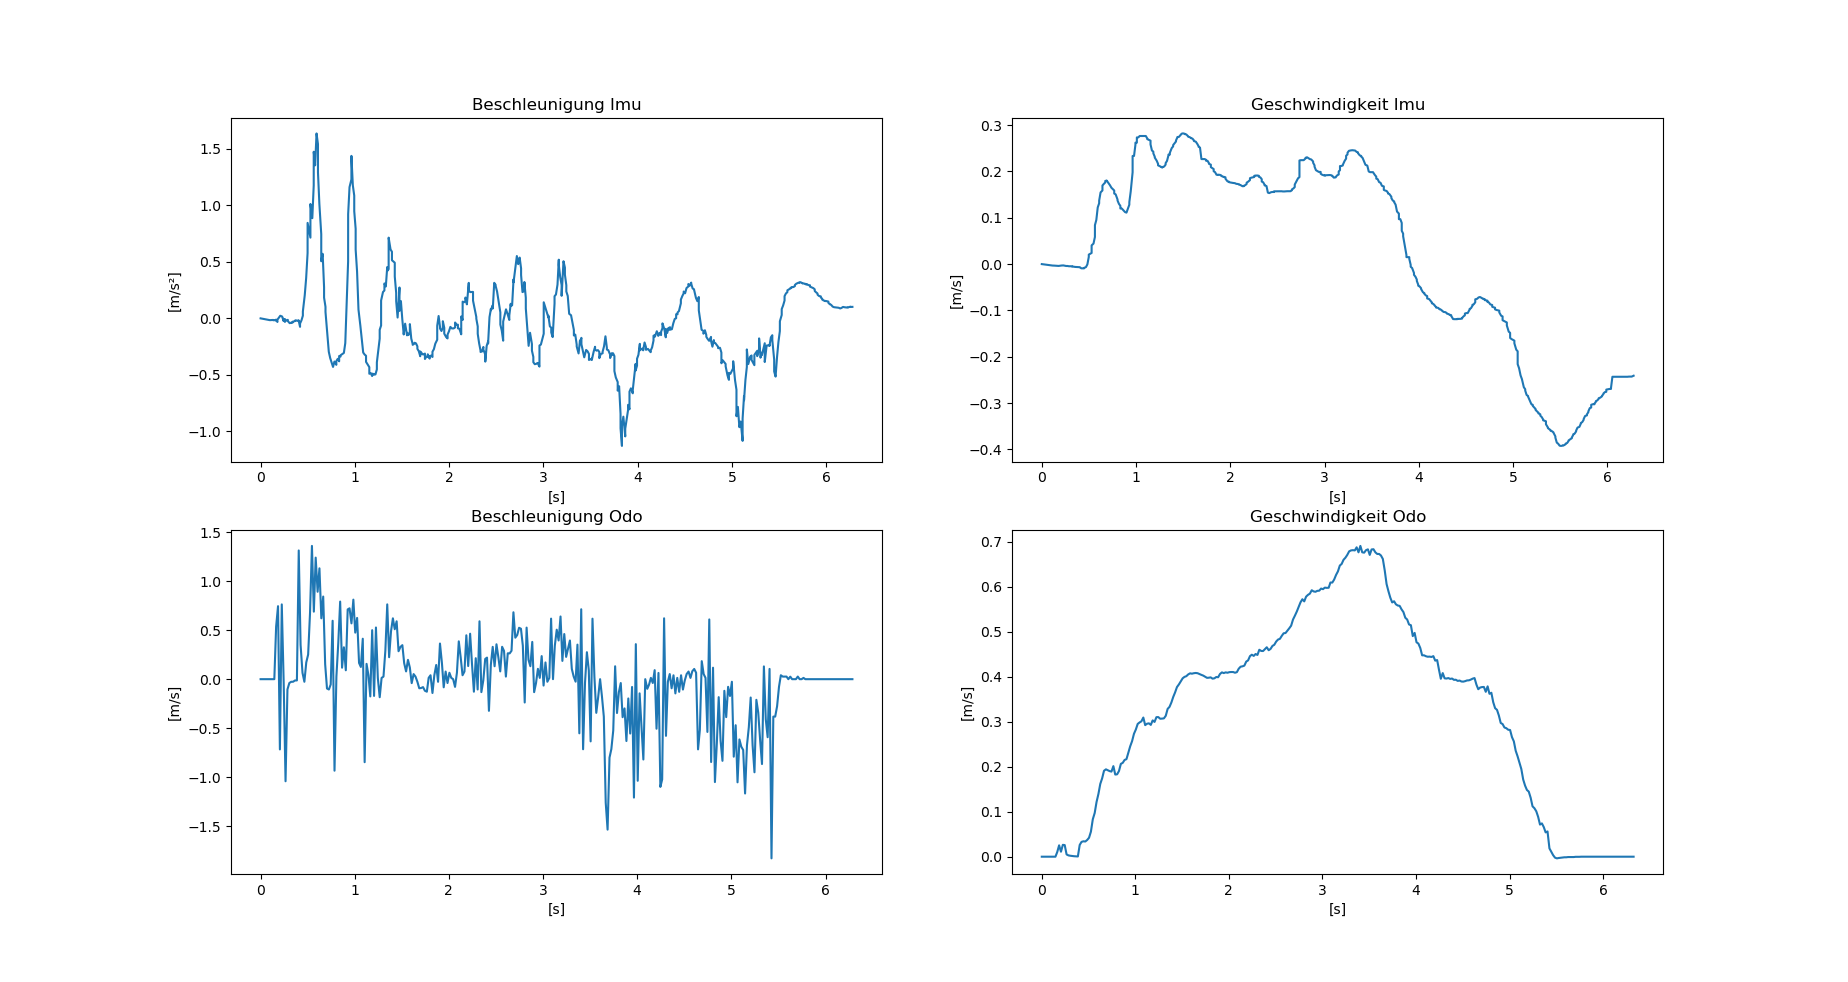
\includegraphics[width=\textwidth]{bilder/23AprImuOdoBeschlGeschw.png}
    \hspace*{-2cm}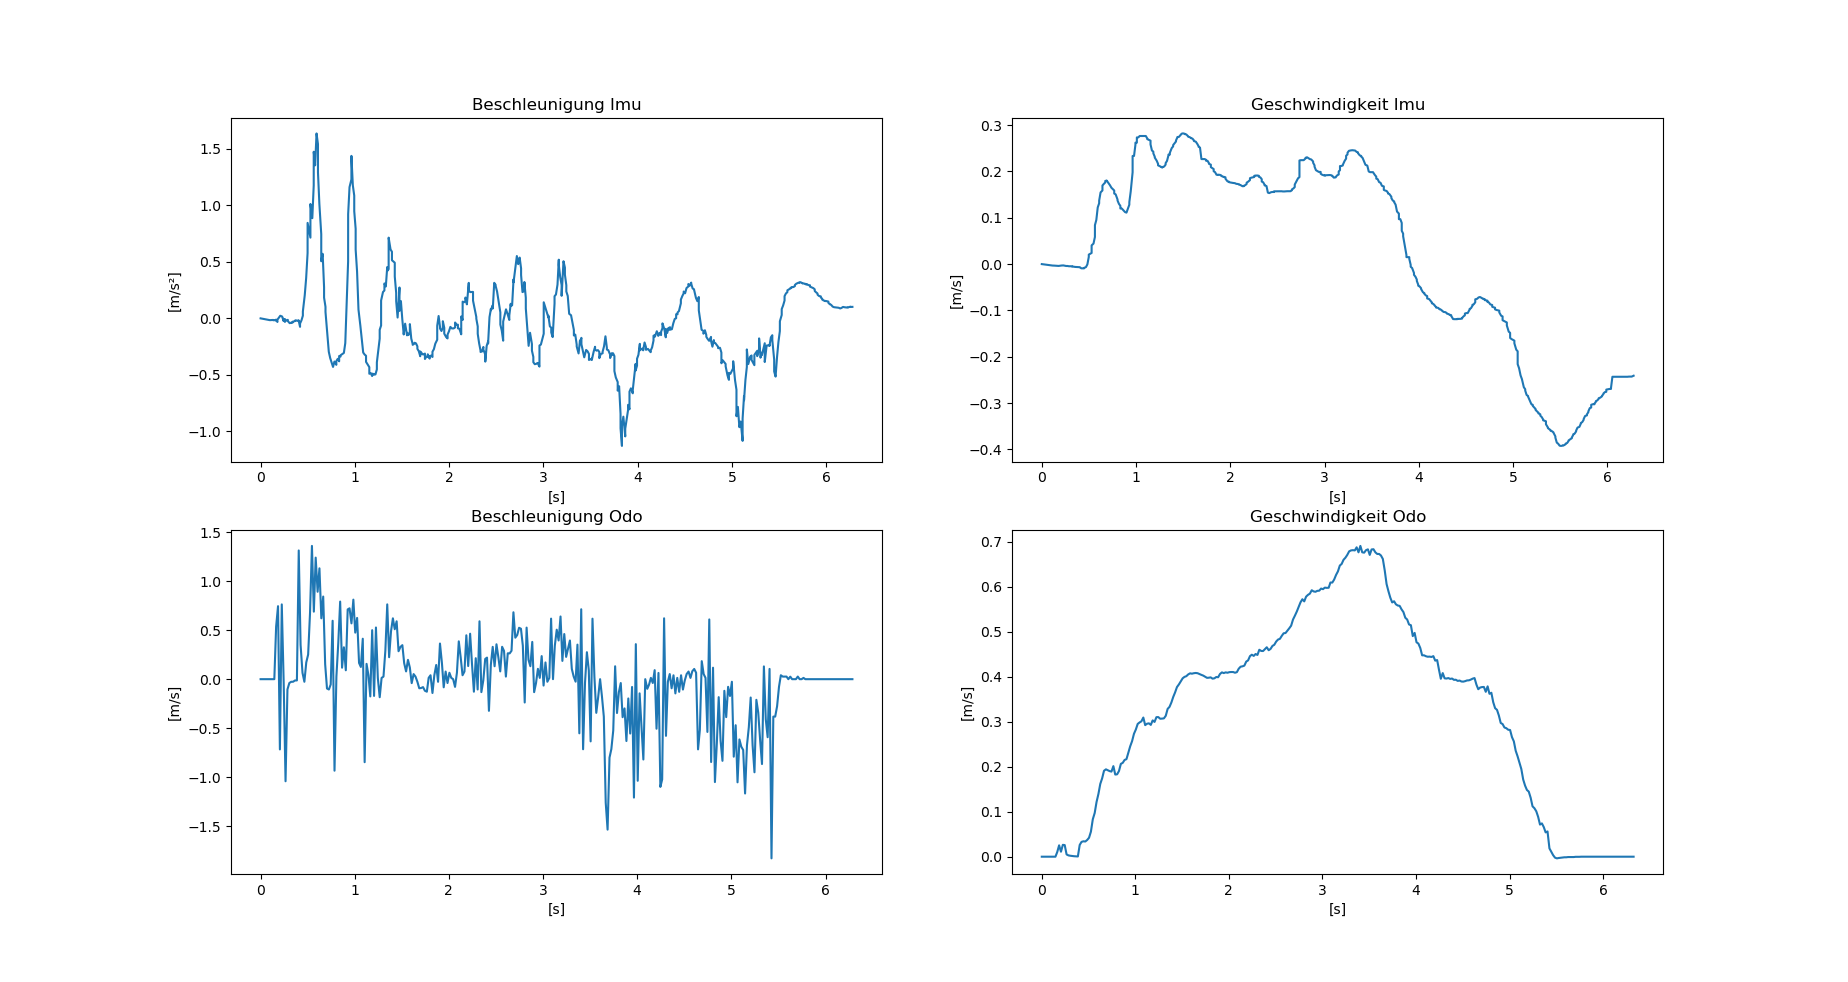
\includegraphics[width=1.25\linewidth]{bilder/23AprImuOdoBeschlGeschw.png}
    \caption{Einzelne Diagramme der Beschleunigung sowie der Geschwindigkeiten}
    \label{fig:diagramAprImuOdoBeschlGeschw}
\end{figure}

Das Problem wird deutlicher in Bild \ref{fig:diagramAprImuOdoBeschlGeschw}. In der Grafik oben rechts ist das Integrierte Signal der IMU. Obwohl das Fahrzeug, wie in der Ansicht der Odometrie unten rechts klar wird, steht, zeigt die IMU eine negative Geschwindigkeit an. Das Signal der Beschleunigung sieht dagegen zwar deutlich Chaotischer aus, offenbart jedoch zwischen Sekunde 5 und 6, dass die Odometrie und die IMU gerade in Extremen werten nicht gleich sind. Tatsächlich drehen die Reifen sich in diesem Szenario durch und die Beschleunigung der Odometrie zeigt nicht die tatsächliche Beschleunigung des Fahrzeugs, sondern nur die erwartete Beschleunigung aufgrund der Geschwindigkeit der Reifen. 

Der Aufbau eines Reglers kann erst stattfinden, wenn die Software diesen Werten vertrauen kann. Damit ist gemeint, dass die Überprüfung der Werte unerlässlich ist. 

\begin{lstlisting}
    sec: 1672855594
    nanosec: 699926525
    sec: 1672855594
    nanosec: 715770401
    sec: 1672855594
    nanosec: 731787777
    sec: 1672855594
    nanosec: 731886526
    sec: 1672855594
    nanosec: 747749124
    sec: 1672855594
    nanosec: 764142540
    sec: 1672855594
    nanosec: 764315234
    sec: 1672855594
    nanosec: 779952251
\end{lstlisting}

Zudem ist das \strong{imu\_transformer} Paket, das es von ROS gestellt gibt, dazu in der Lage die IMU Software-Seitig zu drehen. Sodass sie mit der x-Achse nach vorne zeigt und die z-Achse orthogonal vom Boden weg zeigt. Hierdurch ist es einfacher für Menschen, Lineare Kräfte von Angularen zu Unterscheiden.

\begin{figure}
    \centering
    \hspace*{-2cm}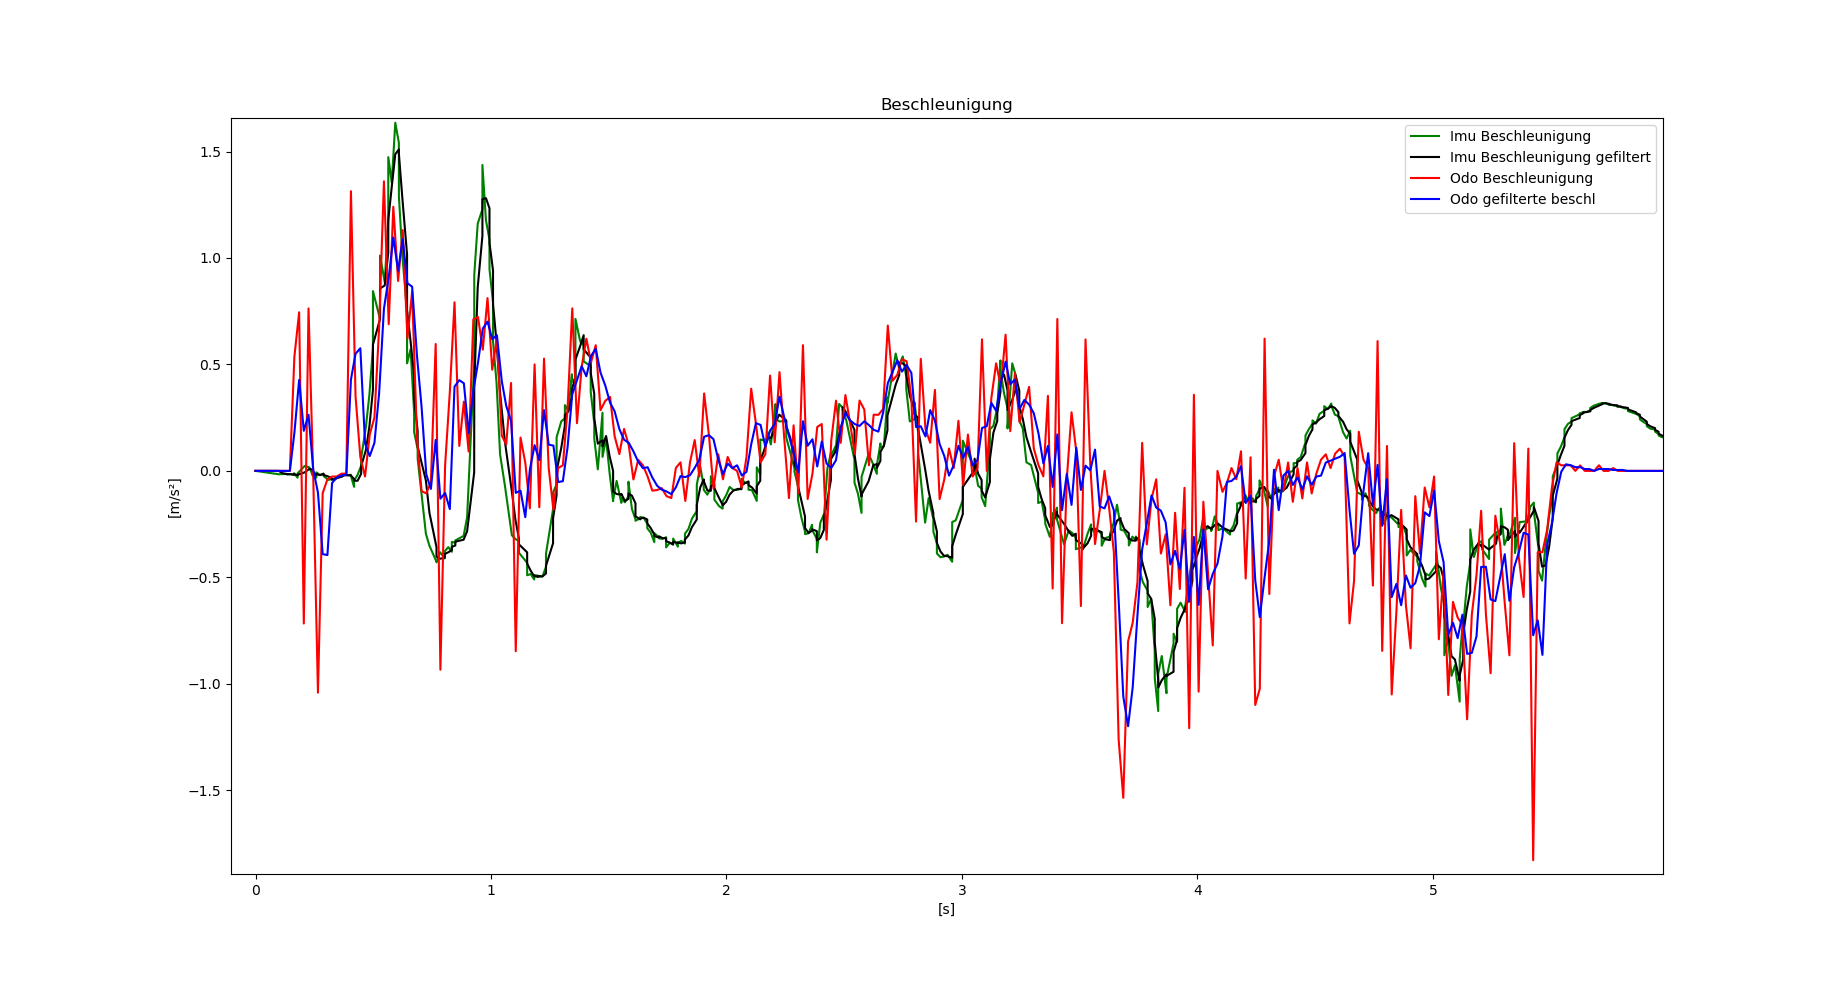
\includegraphics[width=1.2\textwidth]{bilder/23AprBeschlOverlap.png}
    \caption{Beschleunigungswerte übereinander gelegt aktueller Stand}
    \label{fig:diagramApeBeschlOverlap}
\end{figure}


